% Generated by scripts/publish_workflow_results_to_thesis.py. Do not edit.
\begin{table}[htbp]
\centering
\caption[Quantitative test-set results]{Resultados quantitativos no conjunto de test.}
\label{tab:workflow-internal-metrics}
\begin{tabular}{lrrr}
\hline
Modelo & $\Delta$PSNR (dB) & $\Delta$SSIM & Pacientes \\
\hline
dualhead-023-0.9503-img\_out\_ssim\_hu\_20260903\_152341 & 7.77 & 0.1071 & n/a \\
singlehead-033-0.9511-ssim\_hu\_20260903\_151738 & 7.82 & 0.1081 & n/a \\
singlehead\_20260820\_010521 & 7.74 & 0.1080 & 41 \\
singlehead\_20260820\_005026 & 7.56 & 0.1060 & 41 \\
singlehead\_20260820\_003516 & 7.68 & 0.1063 & 41 \\
singlehead\_20260819\_233621 & 7.70 & 0.1078 & 41 \\
\hline
\end{tabular}
\end{table}


\begin{figure}[htbp]
\centering
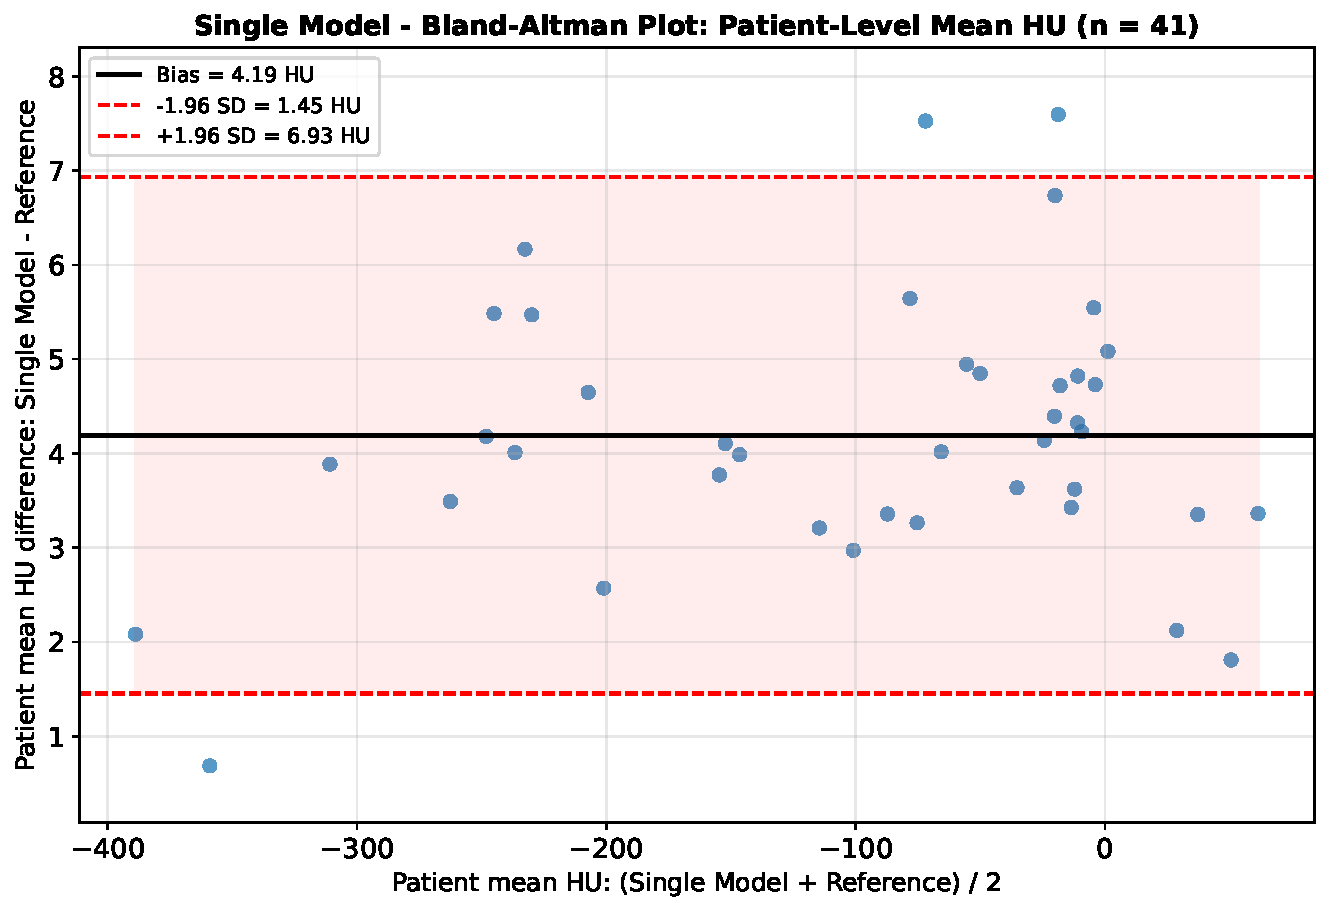
\includegraphics[width=0.95\linewidth]{Figures/Generated/evaluation/bland-altman-45e9e6fa.pdf}
\graphiccaption[Single Model: Bland--Altman plot of patient-level mean HU]{Resultado de avaliacao interna: \texttt{bland\_altman.pdf}.}
\end{figure}

\begin{figure}[htbp]
\centering
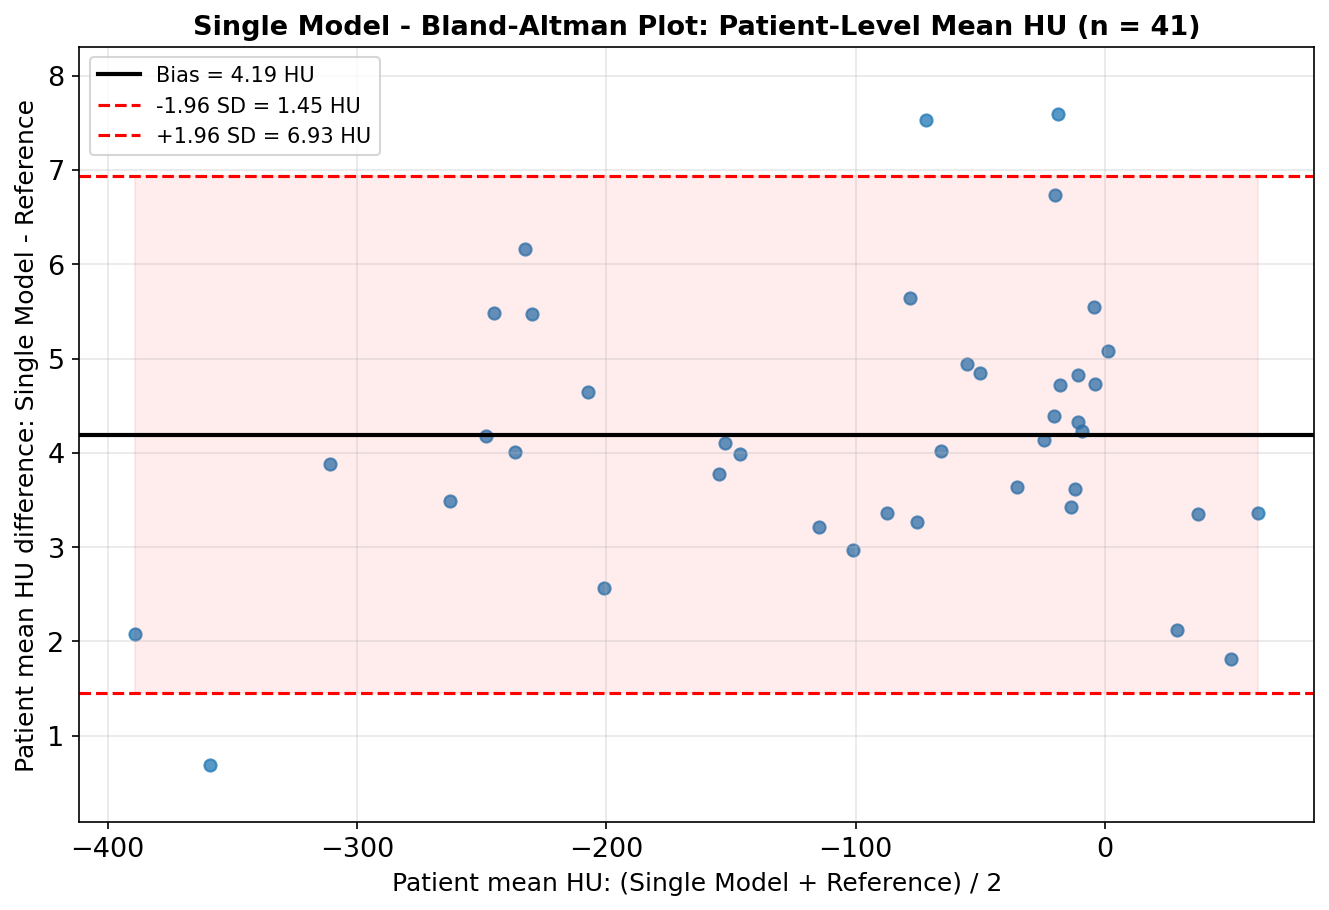
\includegraphics[width=0.95\linewidth]{Figures/Generated/evaluation/bland-altman-5fe9bcb6.png}
\graphiccaption[Single Model: Bland--Altman plot of patient-level mean HU]{Resultado de avaliacao interna: \texttt{bland\_altman.png}.}
\end{figure}

\begin{figure}[htbp]
\centering
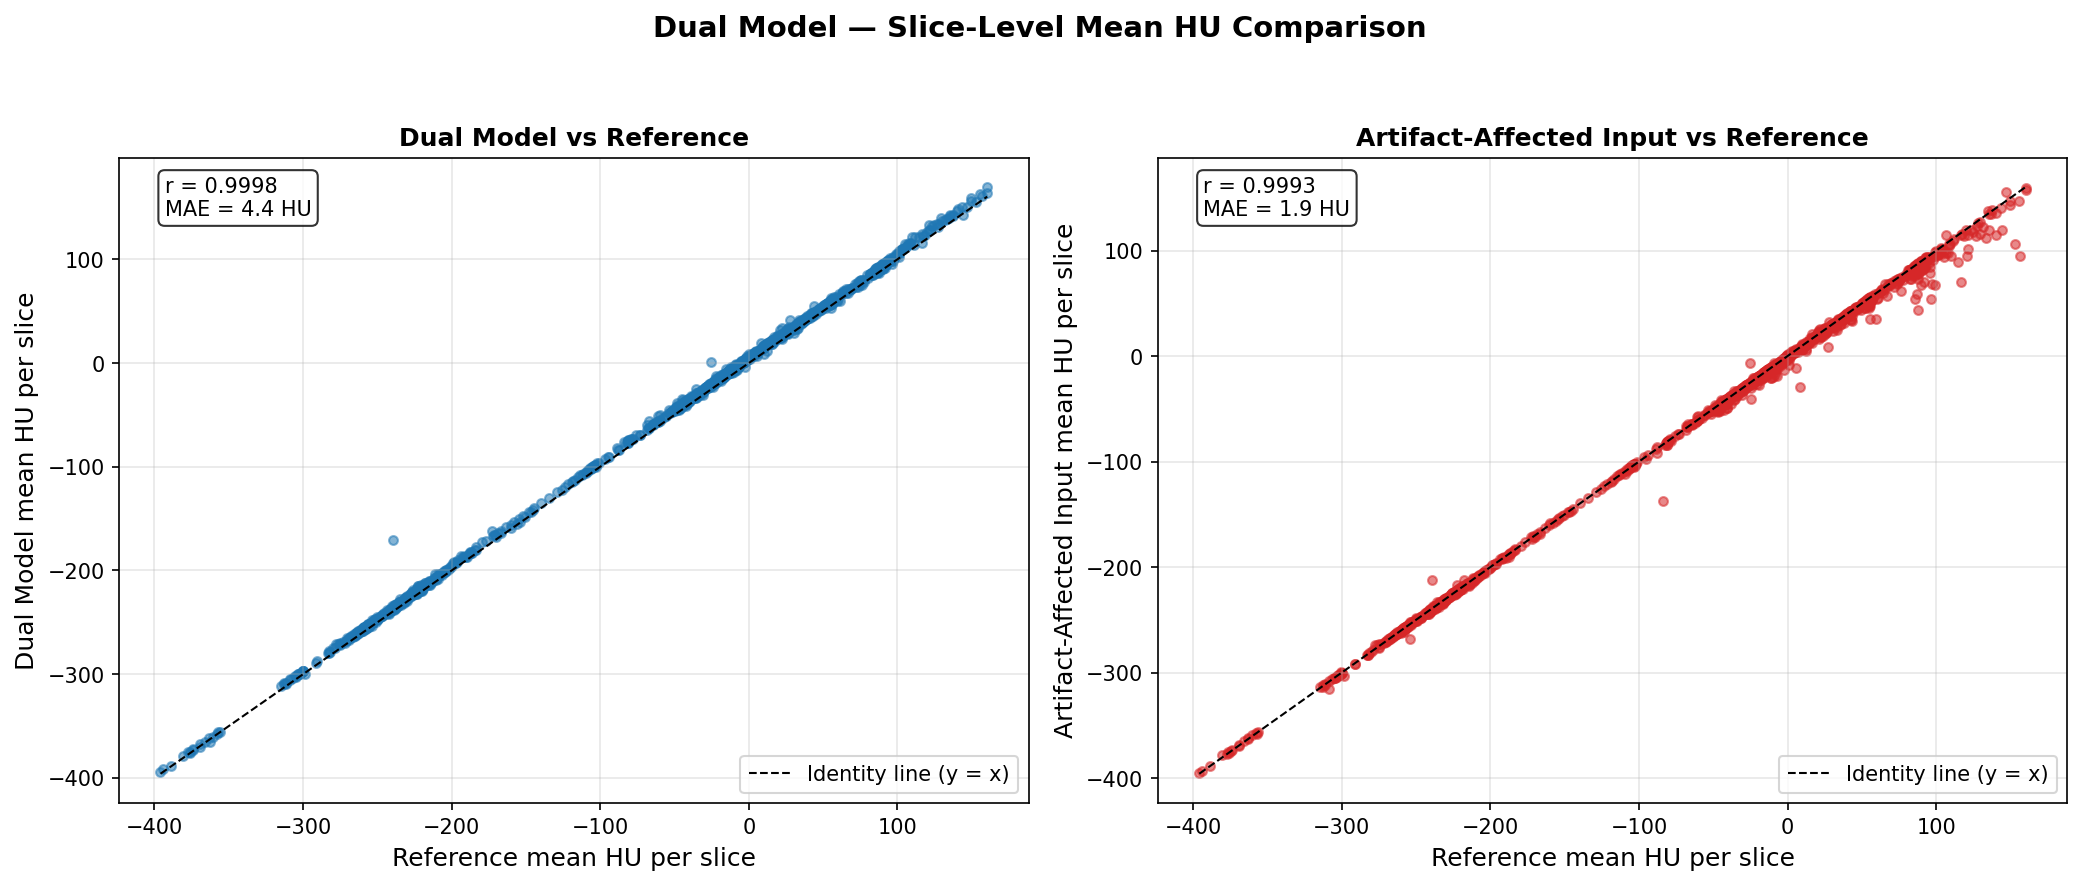
\includegraphics[width=0.95\linewidth]{Figures/Generated/evaluation/scatter-mean-hu-per-slice-c02b1c6c.png}
\graphiccaption[Scatter Mean Hu Per Slice]{Resultado de avaliacao interna: \texttt{scatter\_mean\_hu\_per\_slice.png}.}
\end{figure}

\begin{figure}[htbp]
\centering
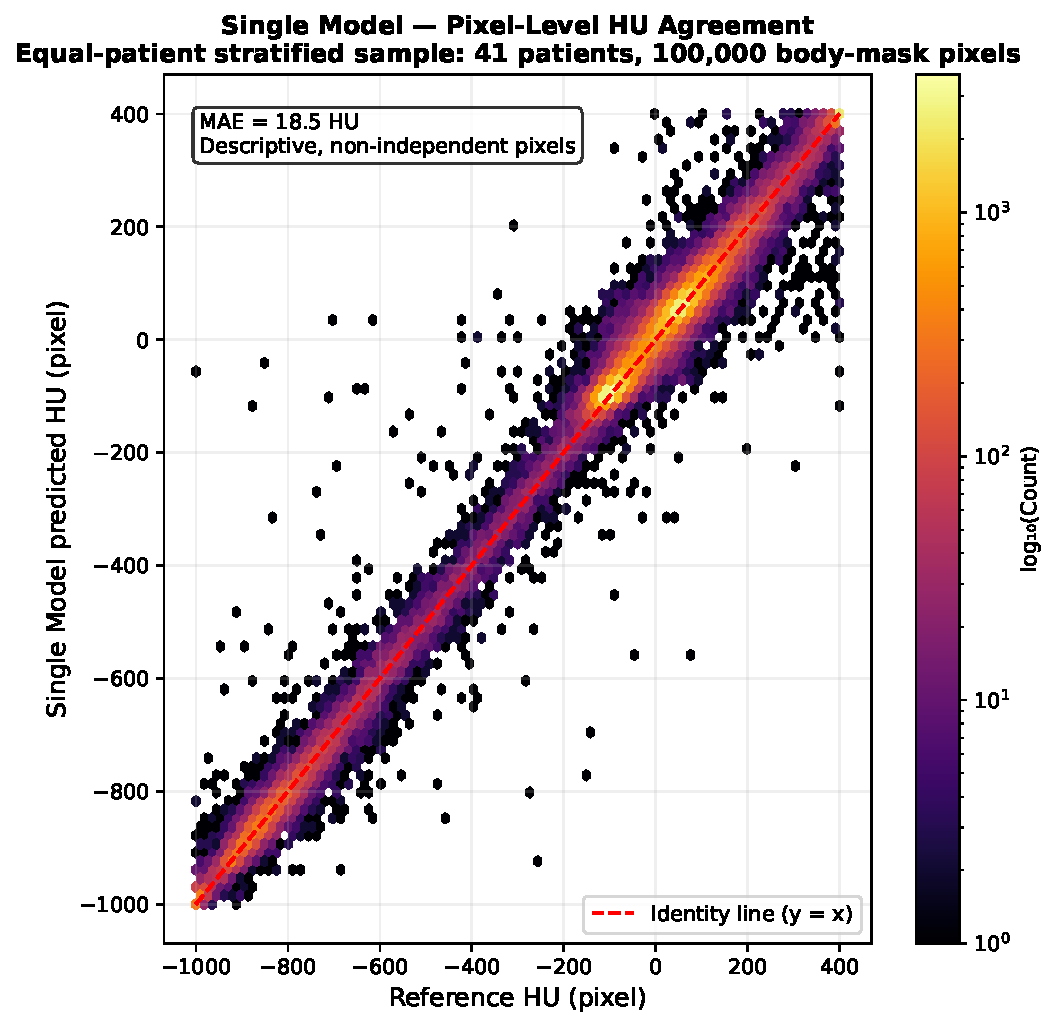
\includegraphics[width=0.95\linewidth]{Figures/Generated/evaluation/scatter-pixel-hu-1396dbc6.pdf}
\graphiccaption[Single Model: pixel-level HU agreement, equal-patient sample]{Resultado de avaliacao interna: \texttt{scatter\_pixel\_hu.pdf}.}
\end{figure}

\begin{figure}[htbp]
\centering
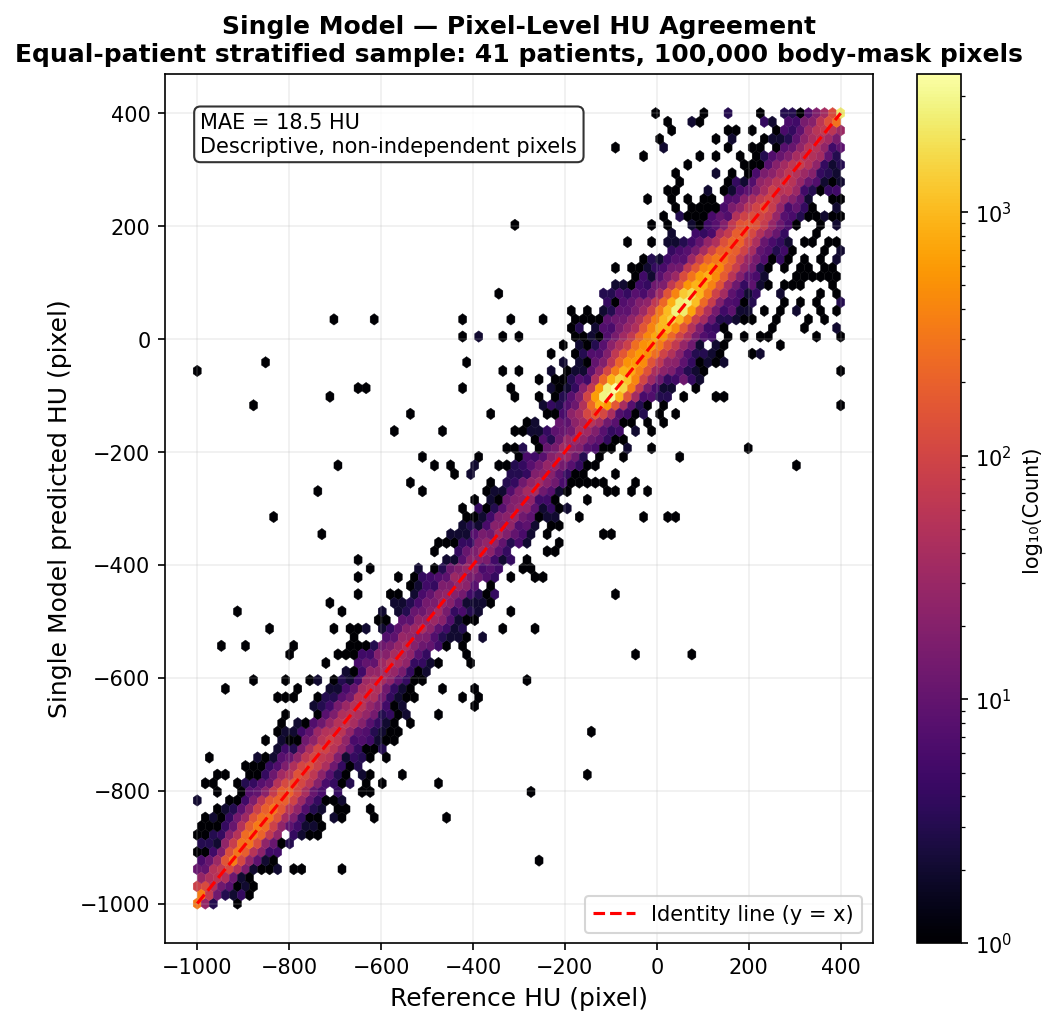
\includegraphics[width=0.95\linewidth]{Figures/Generated/evaluation/scatter-pixel-hu-f5c56e48.png}
\graphiccaption[Single Model: pixel-level HU agreement, equal-patient sample]{Resultado de avaliacao interna: \texttt{scatter\_pixel\_hu.png}.}
\end{figure}

\begin{figure}[htbp]
\centering
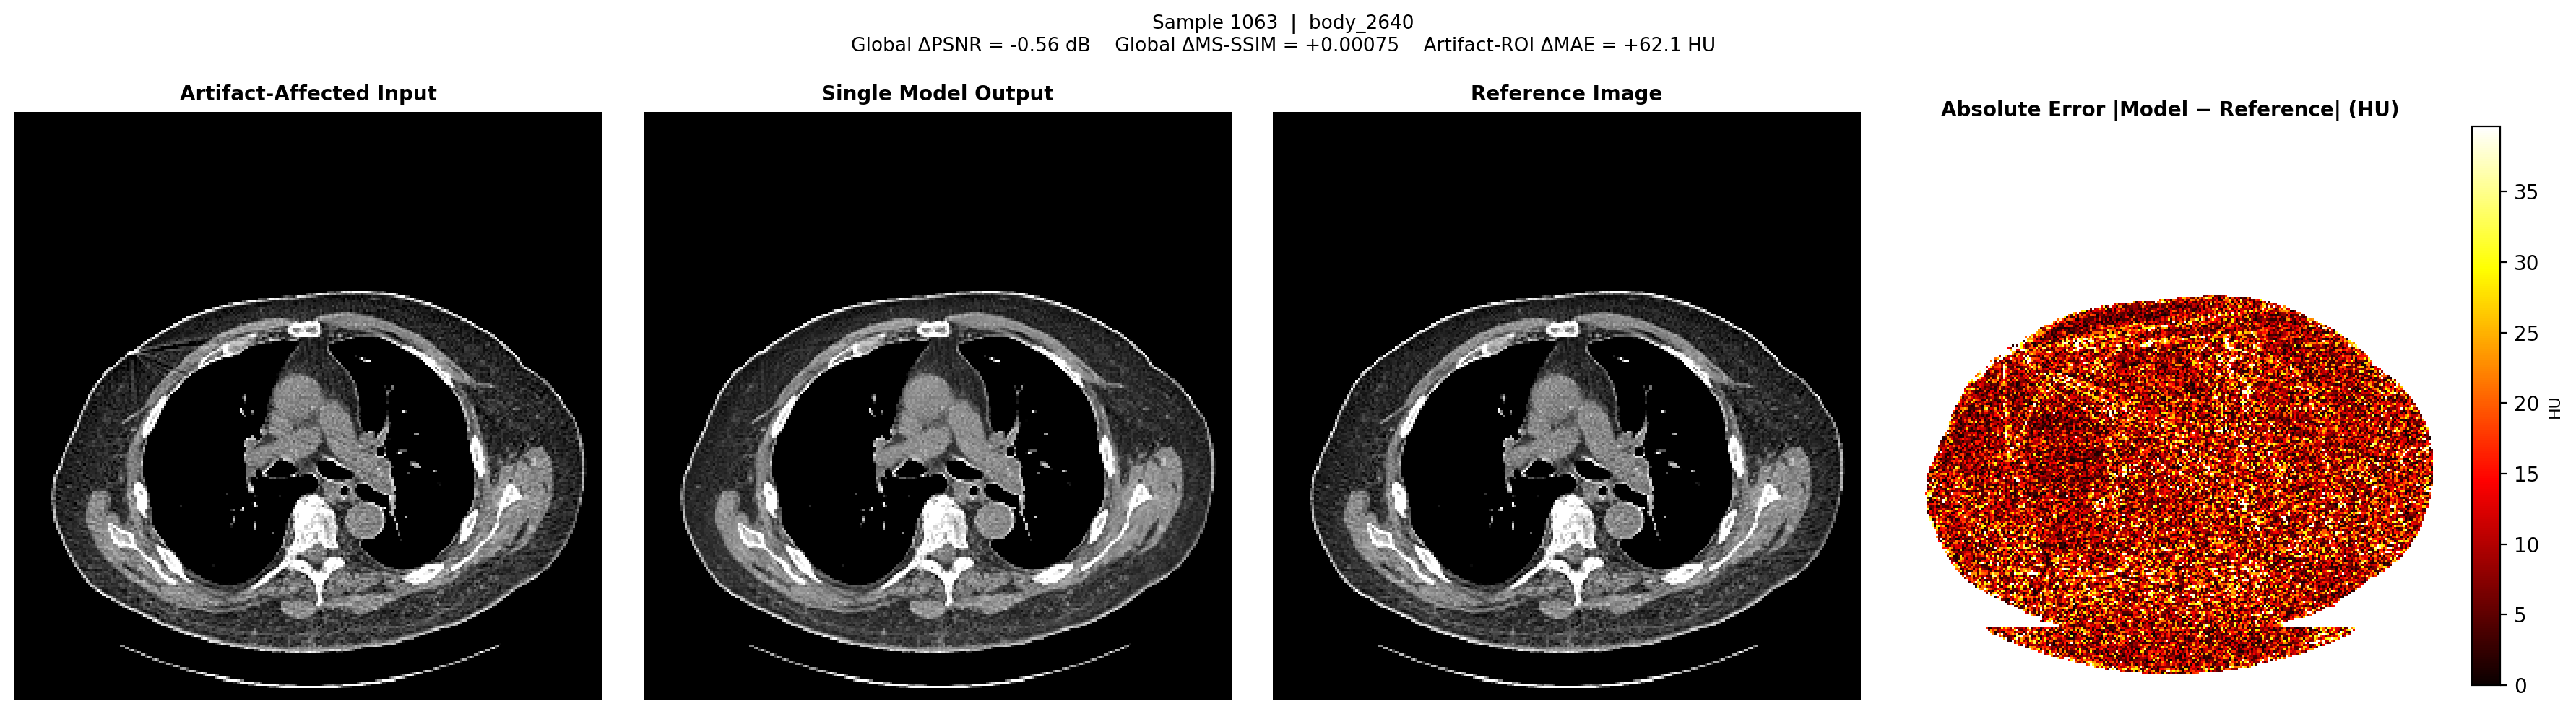
\includegraphics[width=0.95\linewidth]{Figures/Generated/evaluation/pair-1063-body-2640-e5ade870.png}
\caption[Test-set reconstruction example: body pair 1063--2640]{Resultado de avaliacao interna: \texttt{pair\_1063\_body\_2640.png}.}
\end{figure}

\begin{figure}[htbp]
\centering
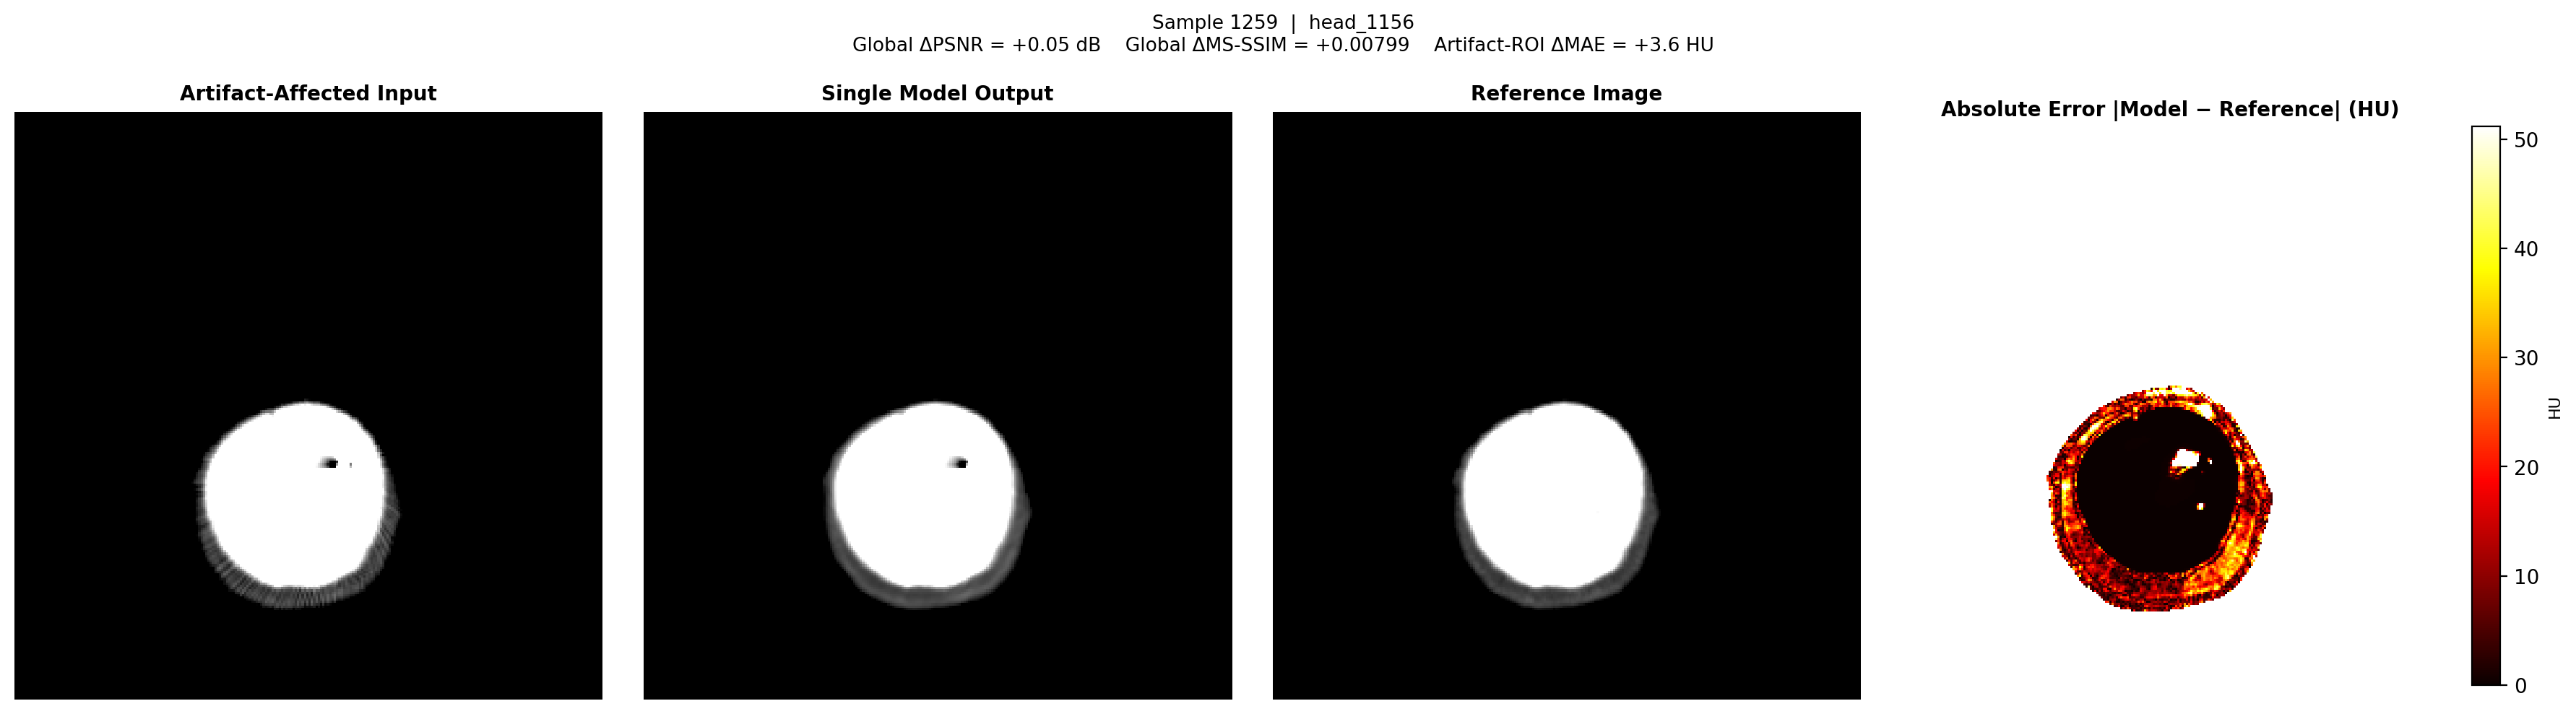
\includegraphics[width=0.95\linewidth]{Figures/Generated/evaluation/pair-1259-head-1156-4339b93b.png}
\caption[Test-set reconstruction example: head pair 1259--1156]{Resultado de avaliacao interna: \texttt{pair\_1259\_head\_1156.png}.}
\end{figure}

\begin{figure}[htbp]
\centering
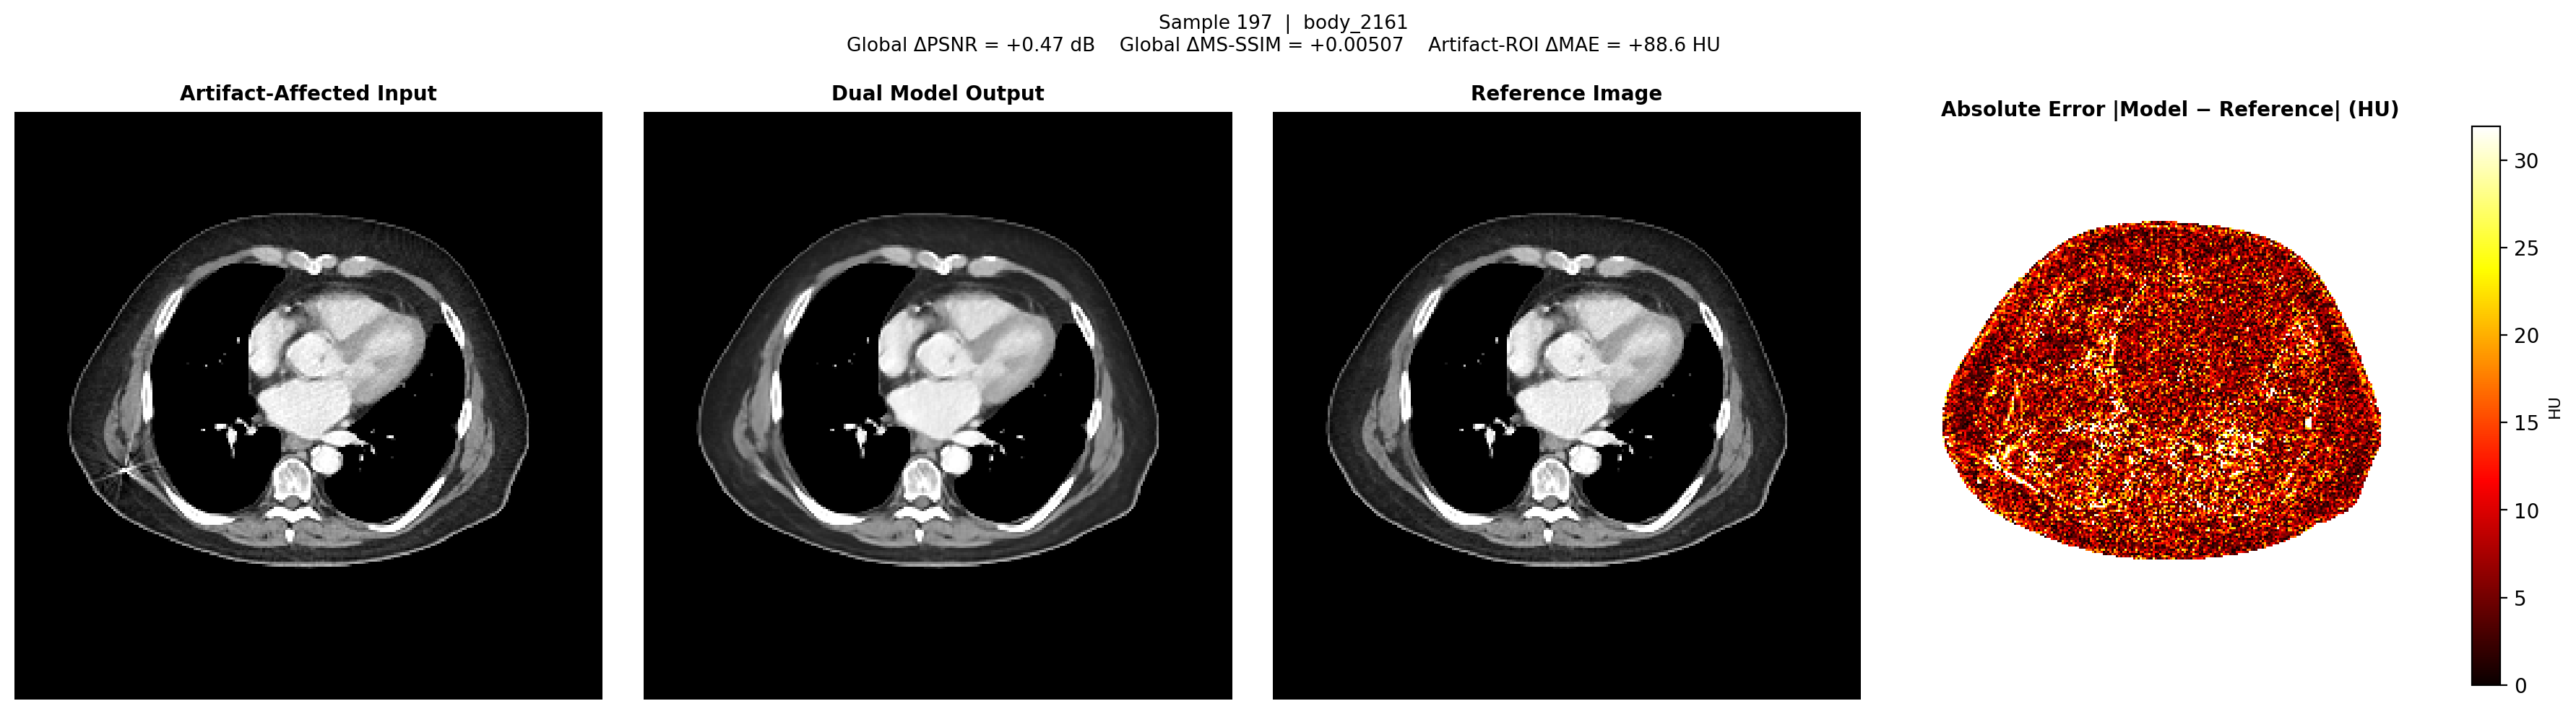
\includegraphics[width=0.95\linewidth]{Figures/Generated/evaluation/pair-197-body-2161-6ac676ec.png}
\caption[Test-set reconstruction example: body pair 197--2161]{Resultado de avaliacao interna: \texttt{pair\_197\_body\_2161.png}.}
\end{figure}

\begin{figure}[htbp]
\centering
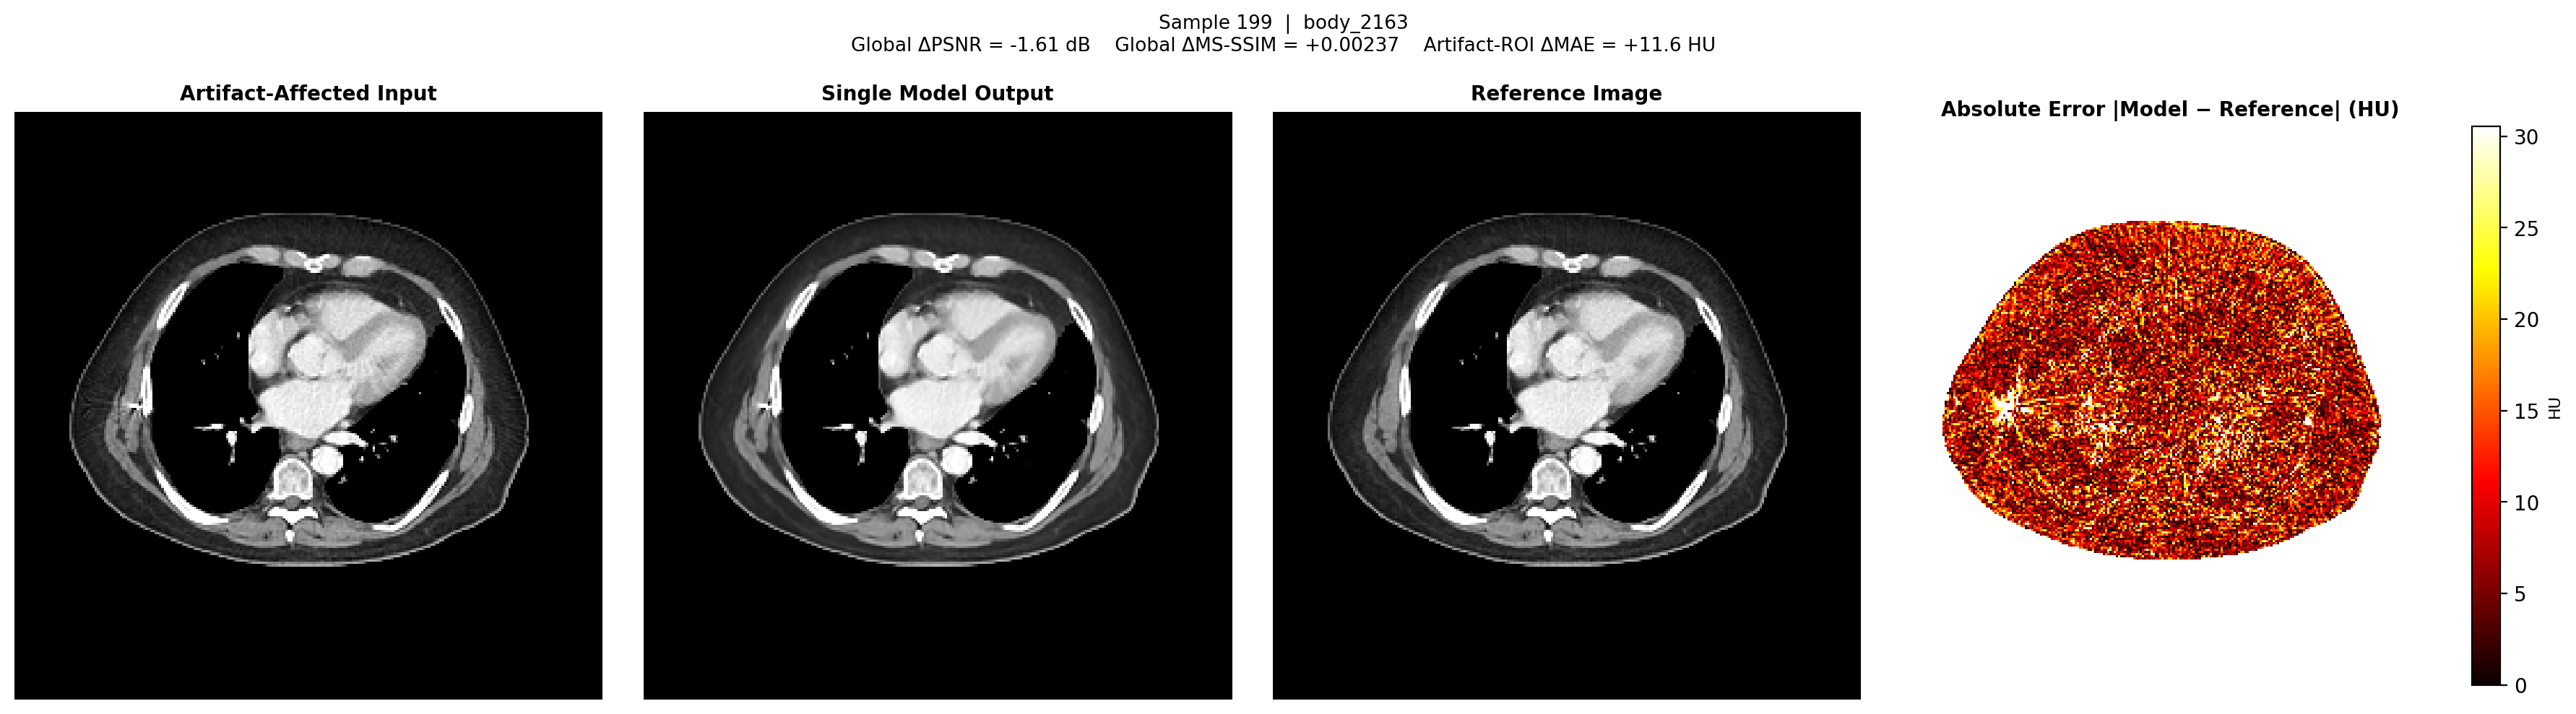
\includegraphics[width=0.95\linewidth]{Figures/Generated/evaluation/pair-199-body-2163-87c95f55.png}
\caption[Test-set reconstruction example: body pair 199--2163]{Resultado de avaliacao interna: \texttt{pair\_199\_body\_2163.png}.}
\end{figure}

\begin{figure}[htbp]
\centering
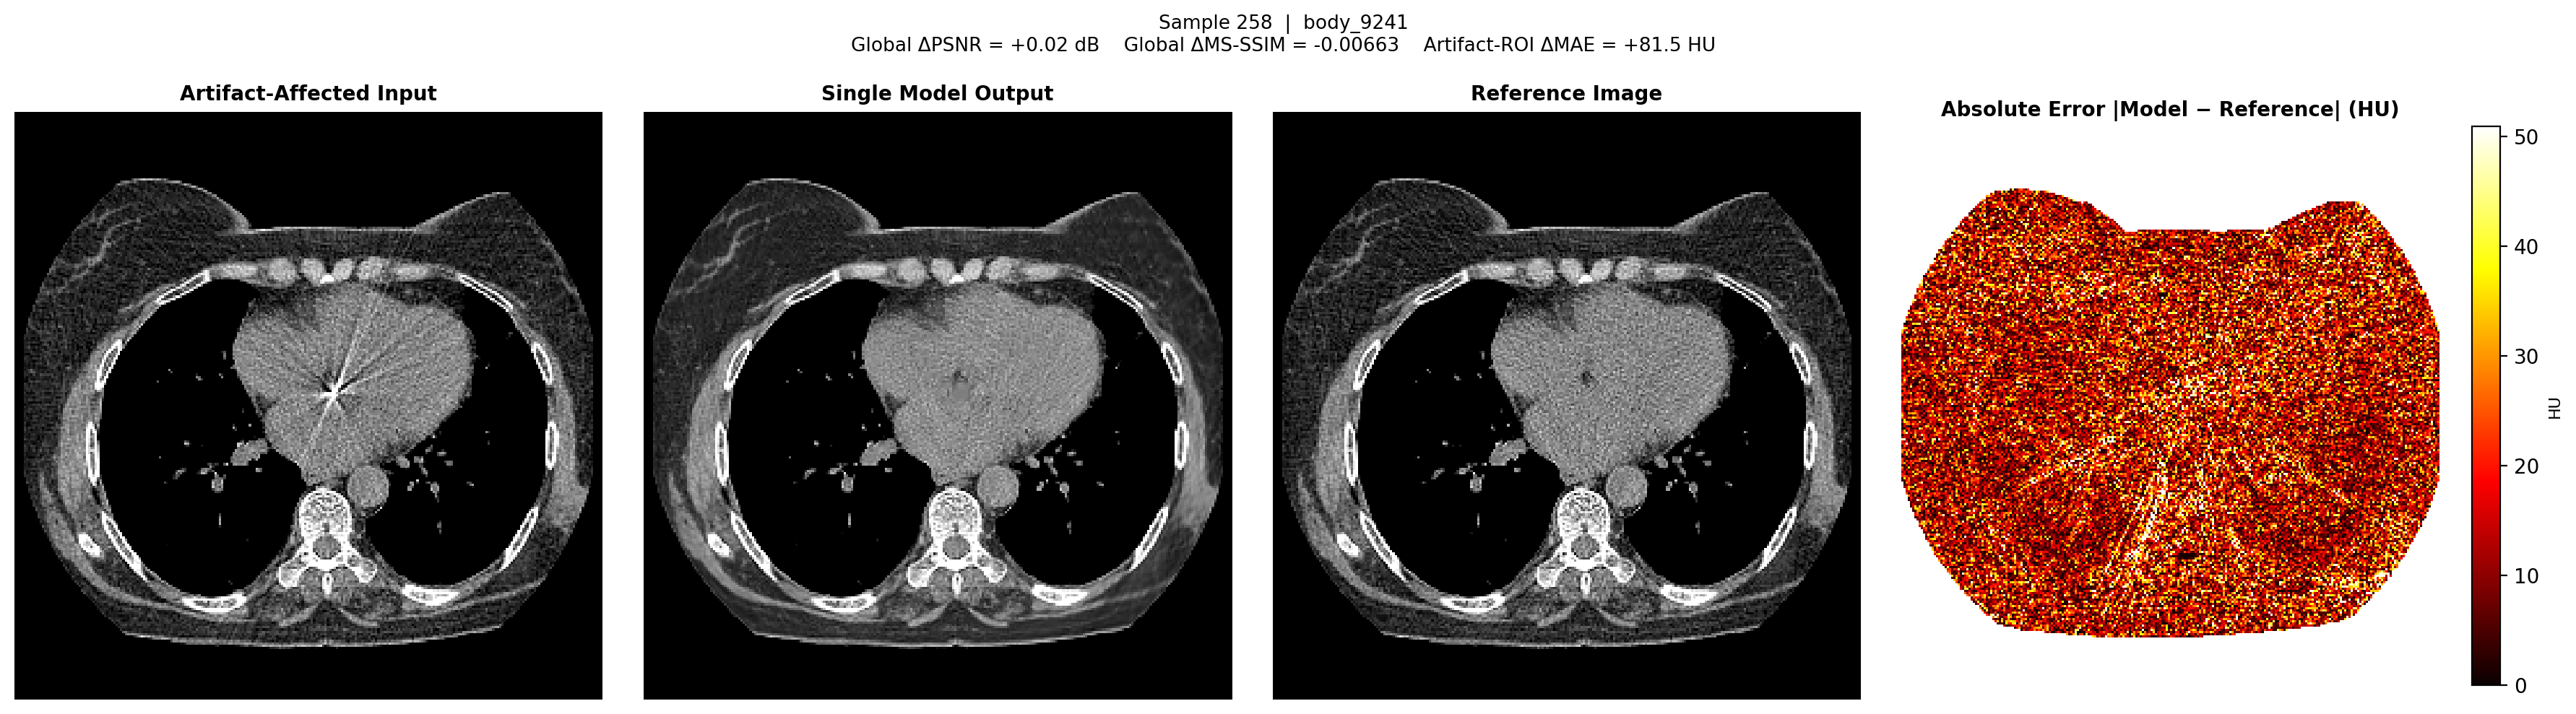
\includegraphics[width=0.95\linewidth]{Figures/Generated/evaluation/pair-258-body-9241-aa56dc98.png}
\caption[Test-set reconstruction example: body pair 258--9241]{Resultado de avaliacao interna: \texttt{pair\_258\_body\_9241.png}.}
\end{figure}

\begin{figure}[htbp]
\centering
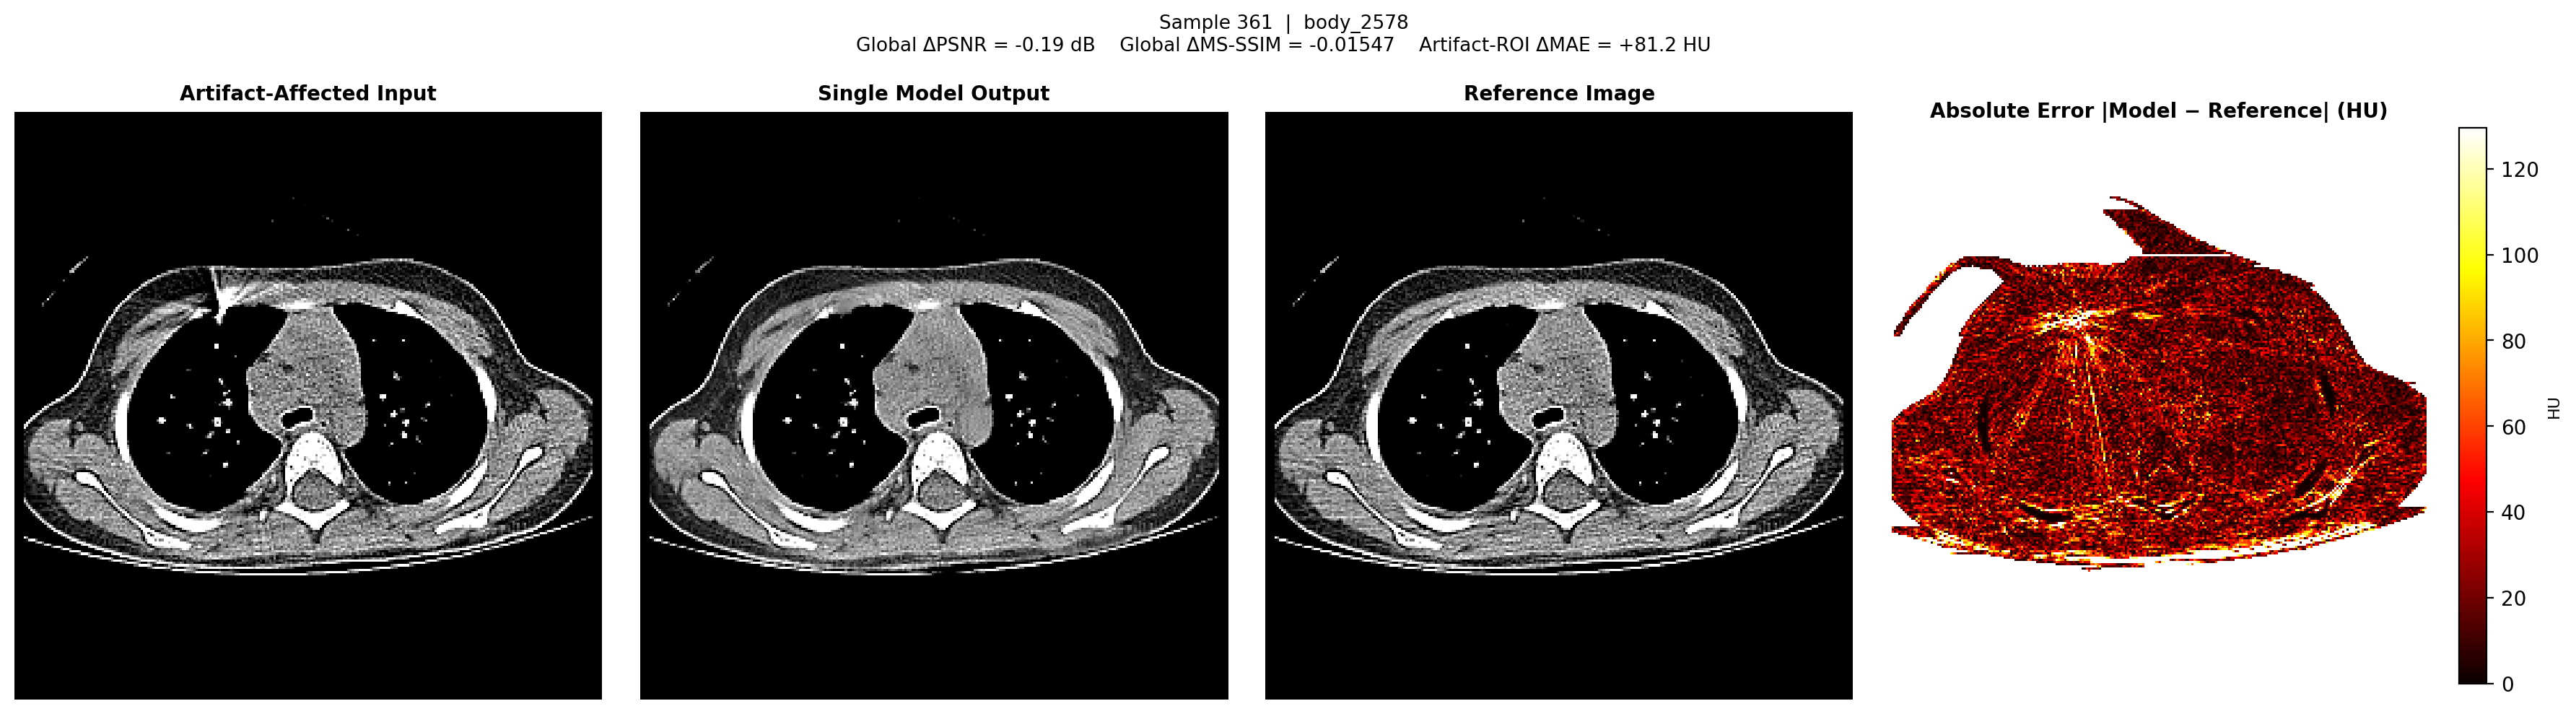
\includegraphics[width=0.95\linewidth]{Figures/Generated/evaluation/pair-361-body-2578-3f506f18.png}
\caption[Test-set reconstruction example: body pair 361--2578]{Resultado de avaliacao interna: \texttt{pair\_361\_body\_2578.png}.}
\end{figure}

% 18 additional copied figure(s) are intentionally not inserted automatically.
\begin{figure}[htbp]
\centering
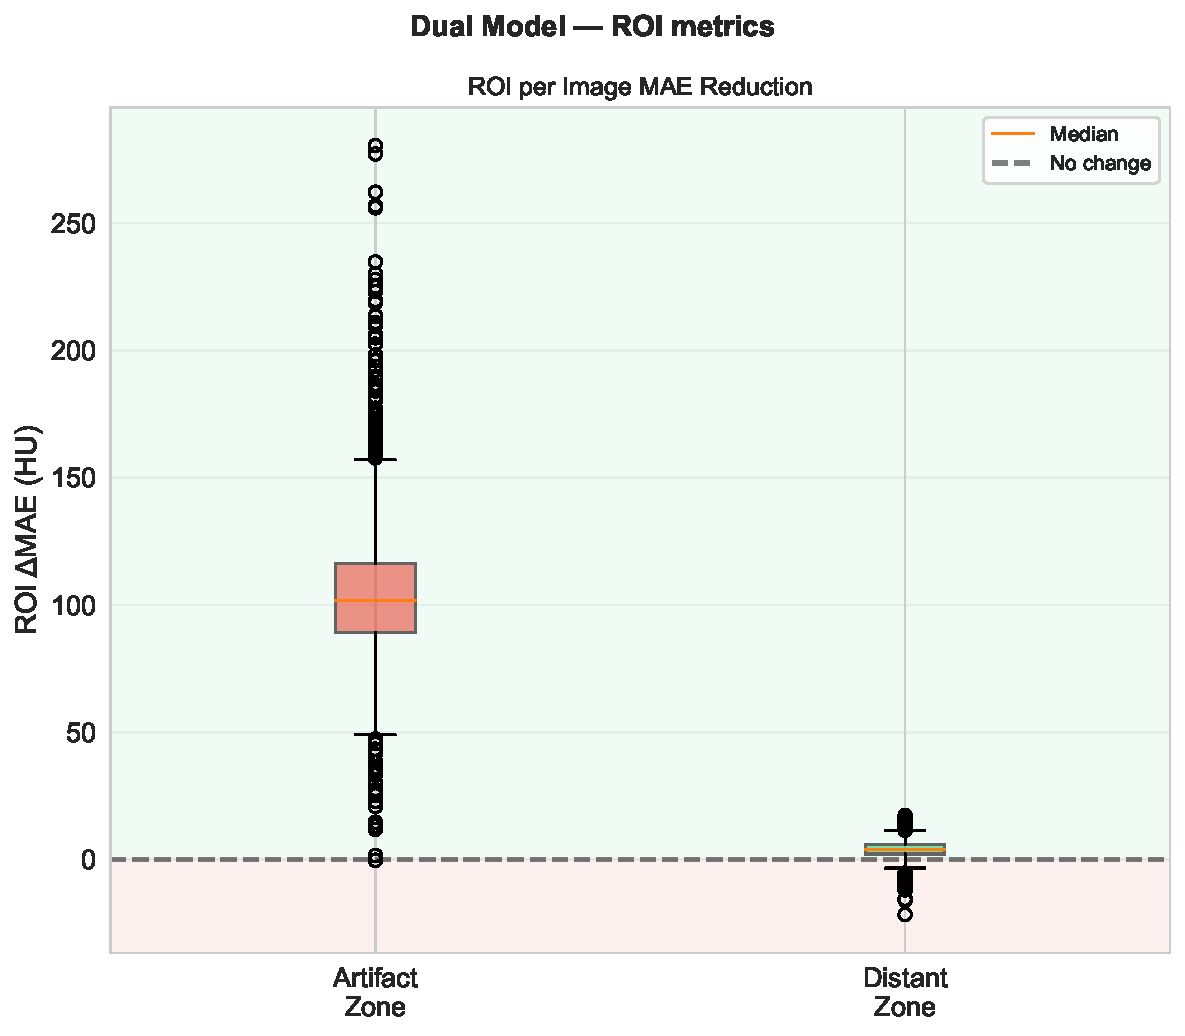
\includegraphics[width=0.95\linewidth]{Figures/Generated/evaluation/boxplot-roi-delta-mae-2809e634.pdf}
\graphiccaption[ROI per-image MAE reduction]{Distribuicao de metricas e analise de correlacao: \texttt{boxplot\_roi\_delta\_mae.pdf}.}
\end{figure}

\begin{figure}[htbp]
\centering
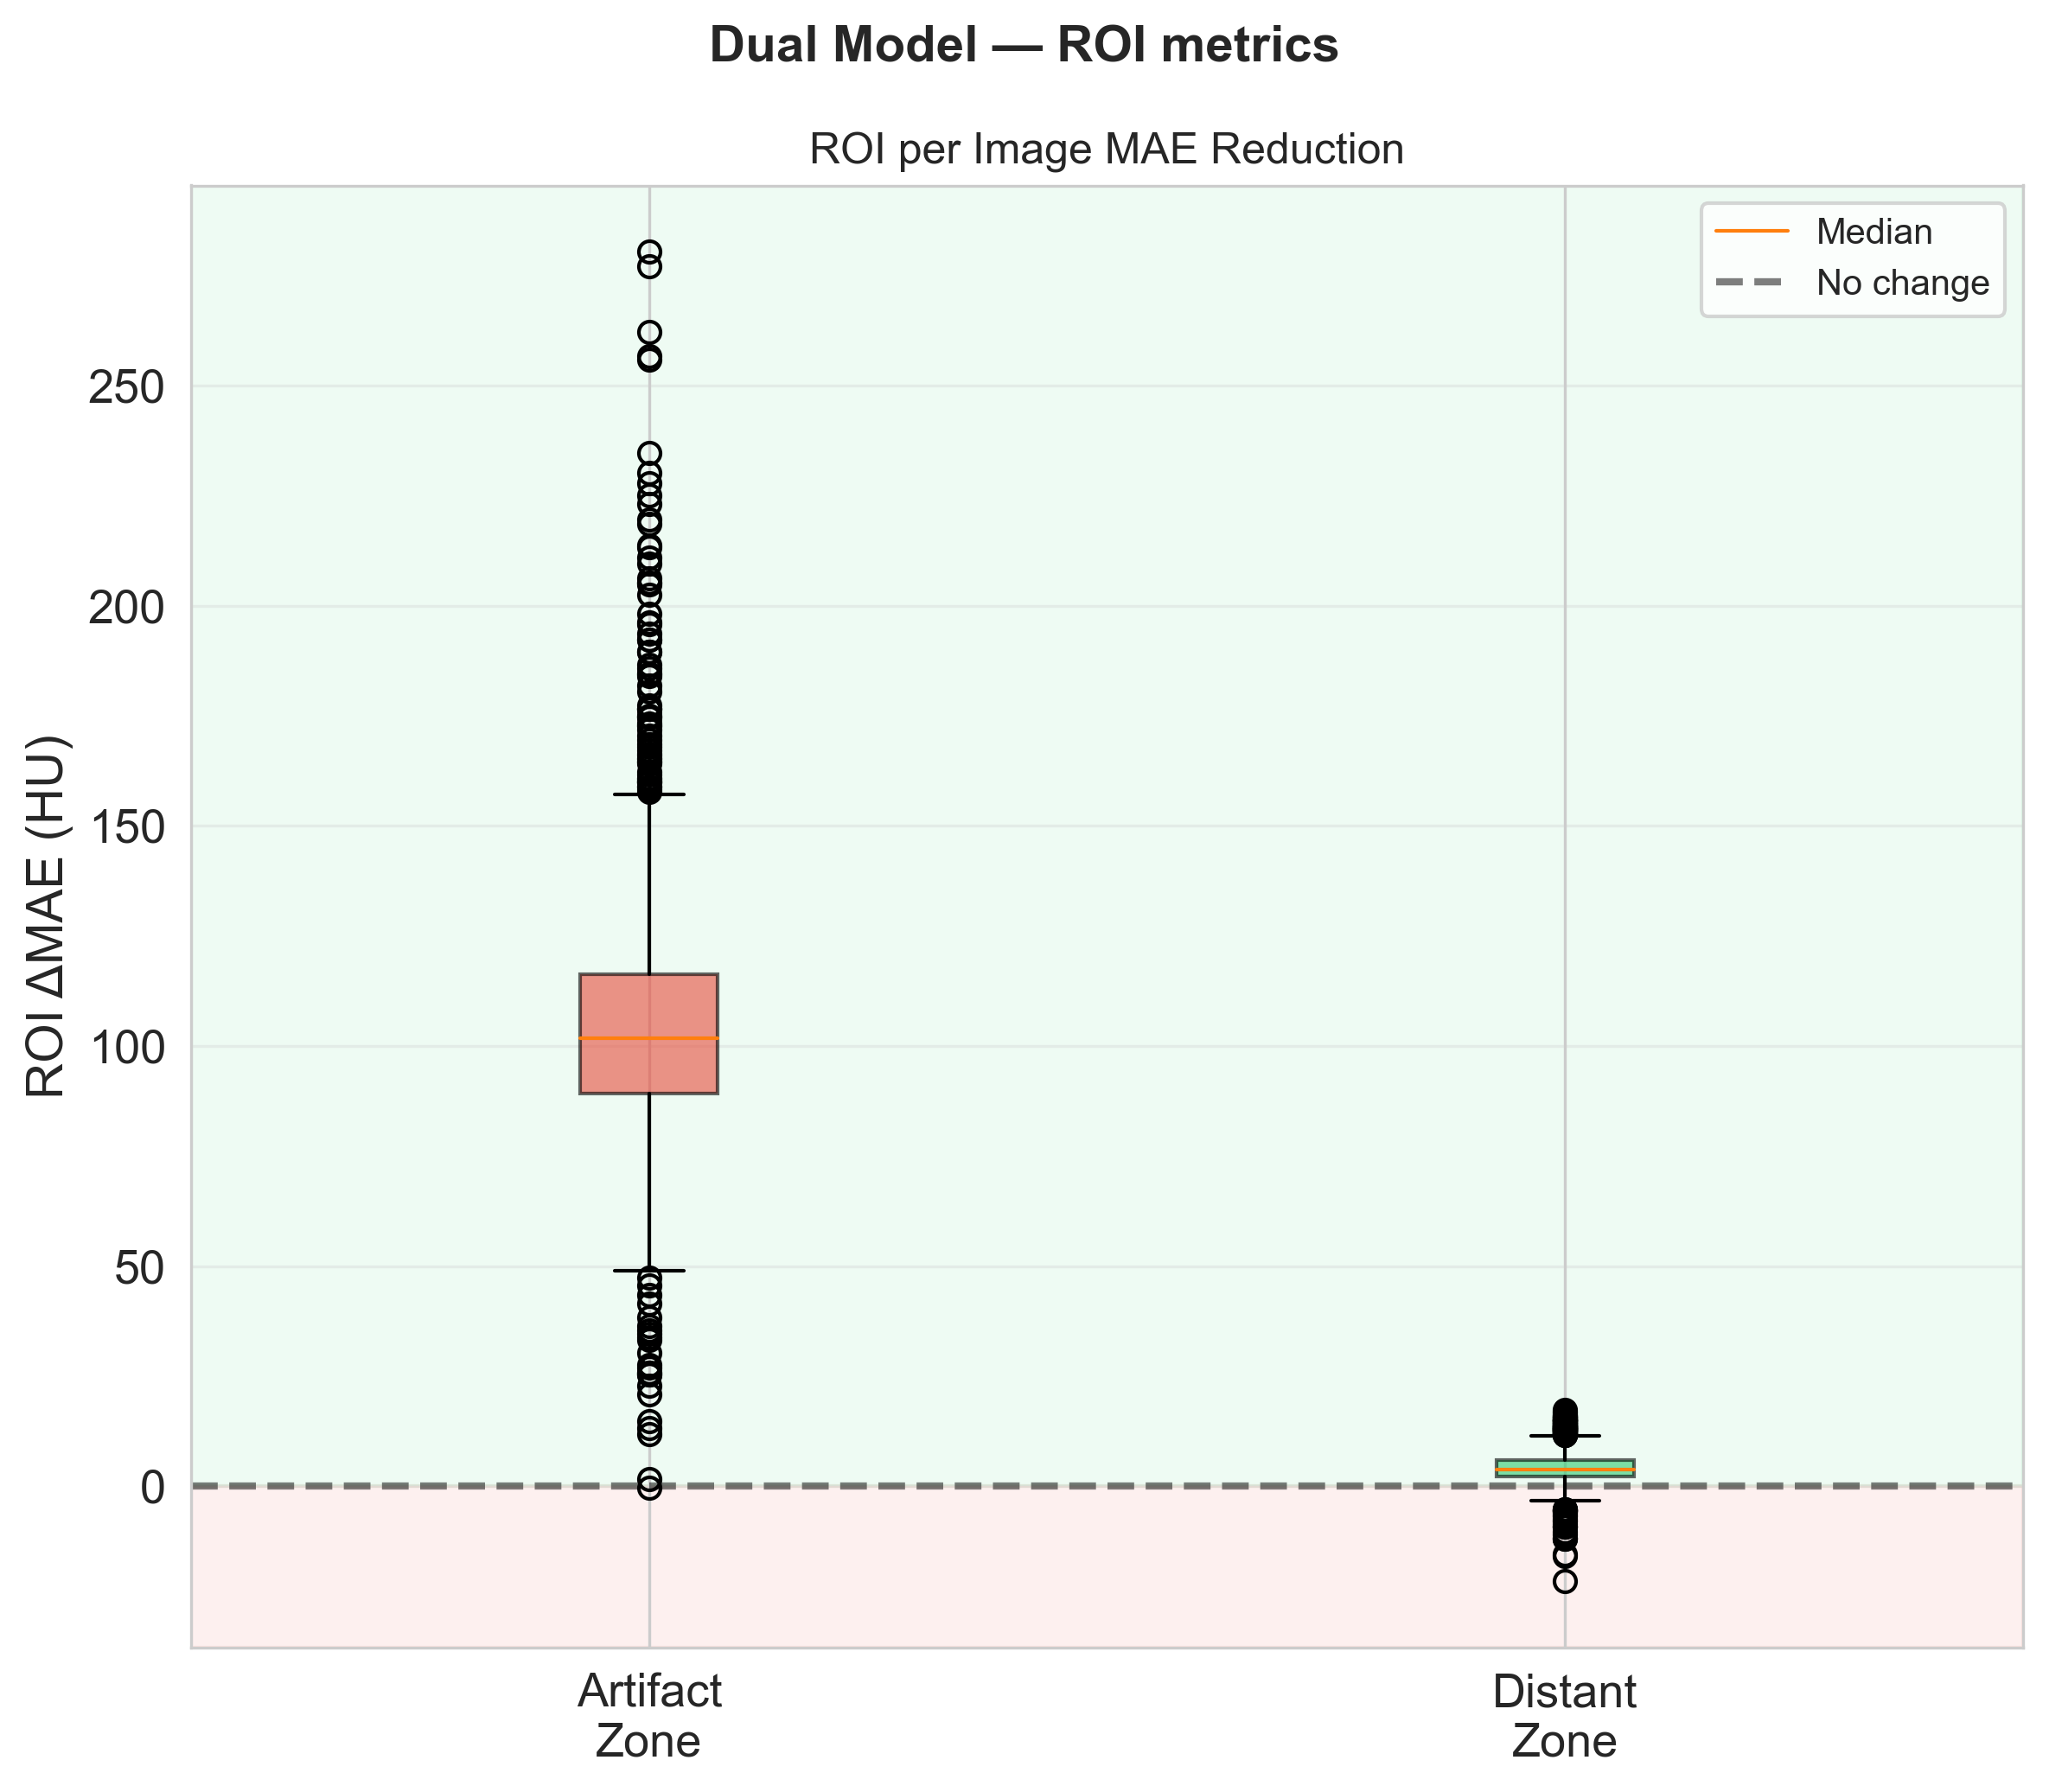
\includegraphics[width=0.95\linewidth]{Figures/Generated/evaluation/boxplot-roi-delta-mae-a69c3ca2.png}
\graphiccaption[ROI per-image MAE reduction]{Distribuicao de metricas e analise de correlacao: \texttt{boxplot\_roi\_delta\_mae.png}.}
\end{figure}

\begin{figure}[htbp]
\centering
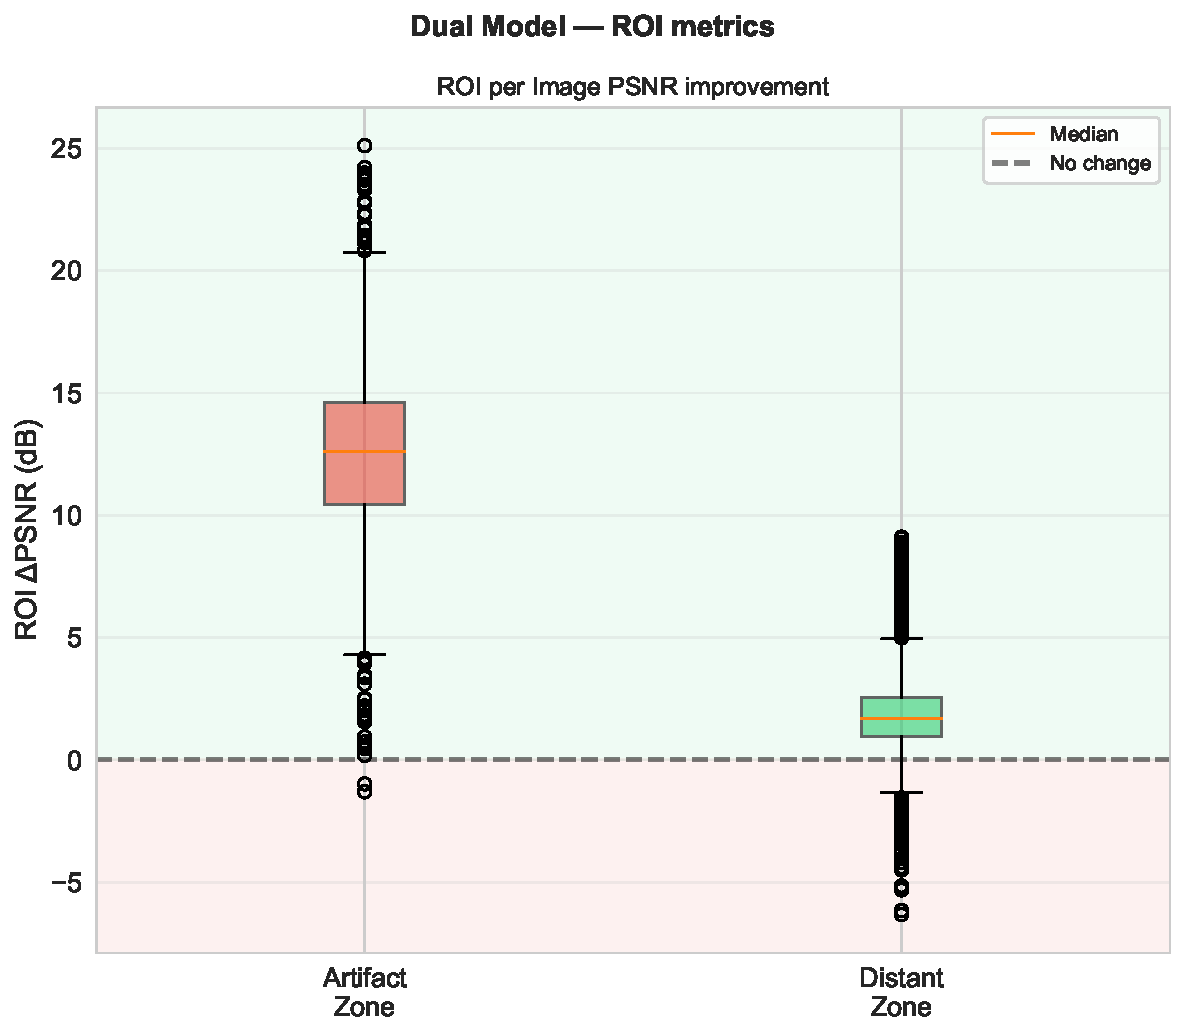
\includegraphics[width=0.95\linewidth]{Figures/Generated/evaluation/boxplot-roi-delta-psnr-014f3a02.pdf}
\graphiccaption[ROI per-image PSNR improvement]{Distribuicao de metricas e analise de correlacao: \texttt{boxplot\_roi\_delta\_psnr.pdf}.}
\end{figure}

\begin{figure}[htbp]
\centering
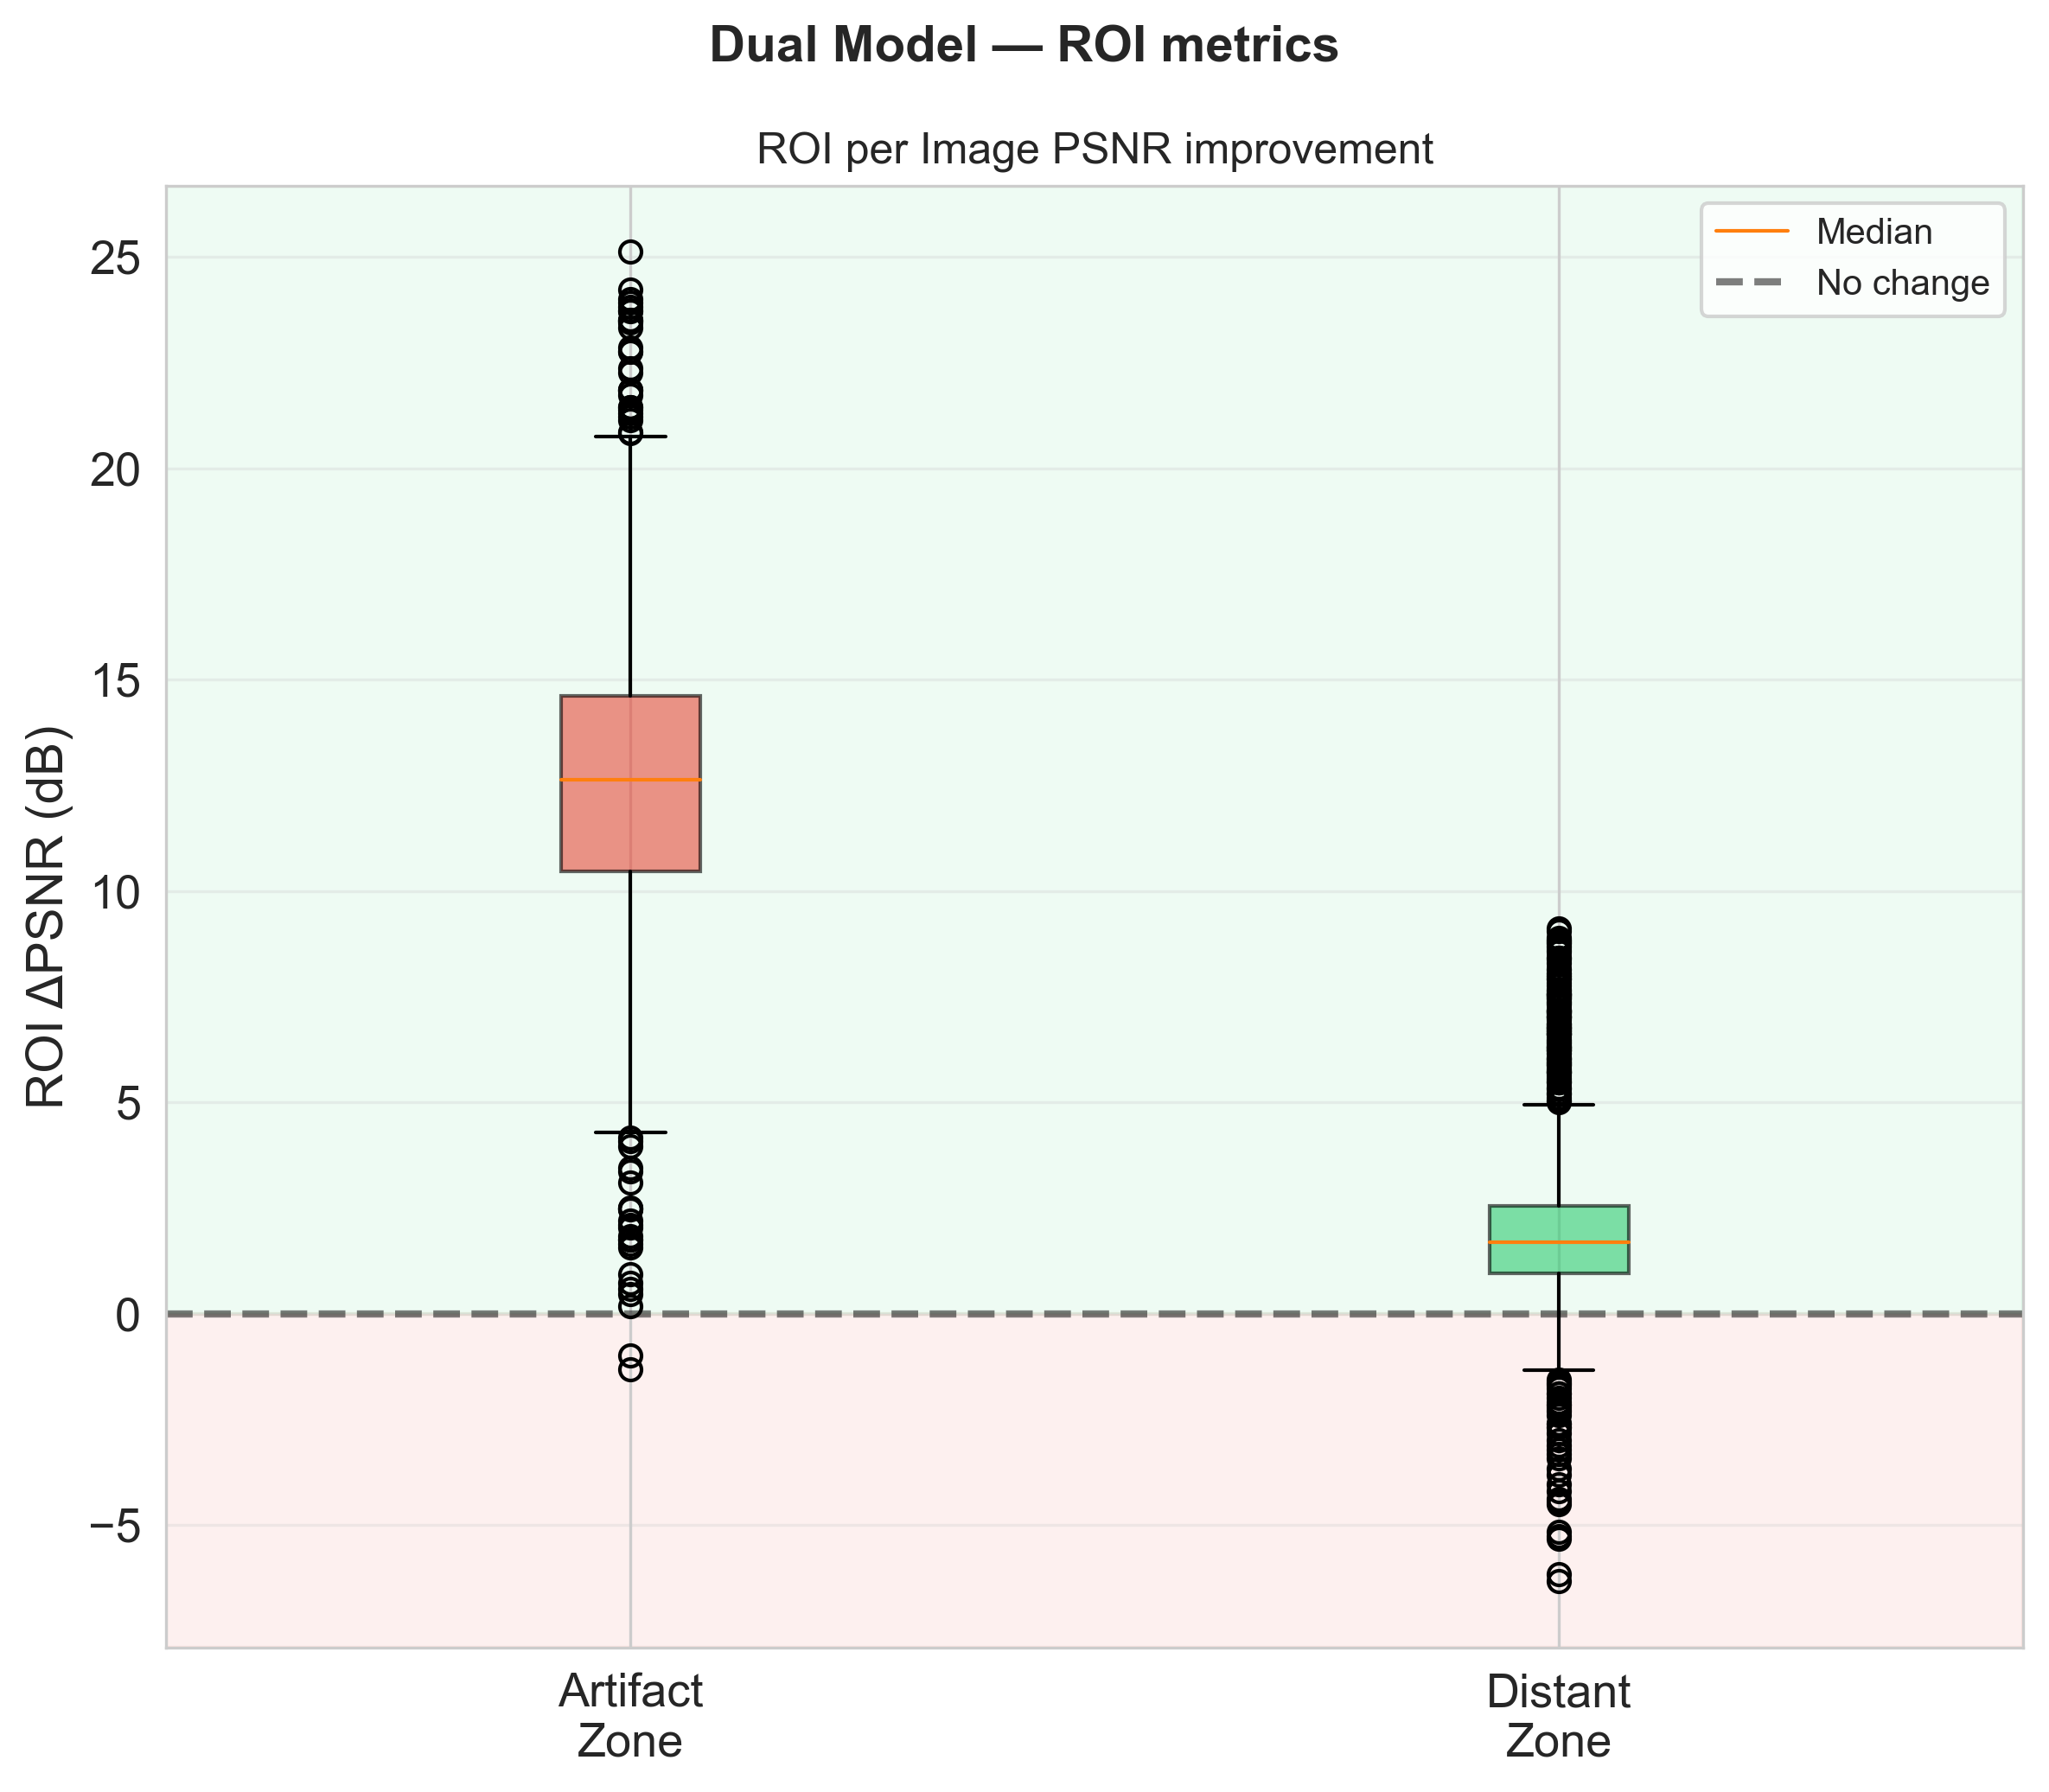
\includegraphics[width=0.95\linewidth]{Figures/Generated/evaluation/boxplot-roi-delta-psnr-89620f8c.png}
\graphiccaption[ROI per-image PSNR improvement]{Distribuicao de metricas e analise de correlacao: \texttt{boxplot\_roi\_delta\_psnr.png}.}
\end{figure}

\begin{figure}[htbp]
\centering
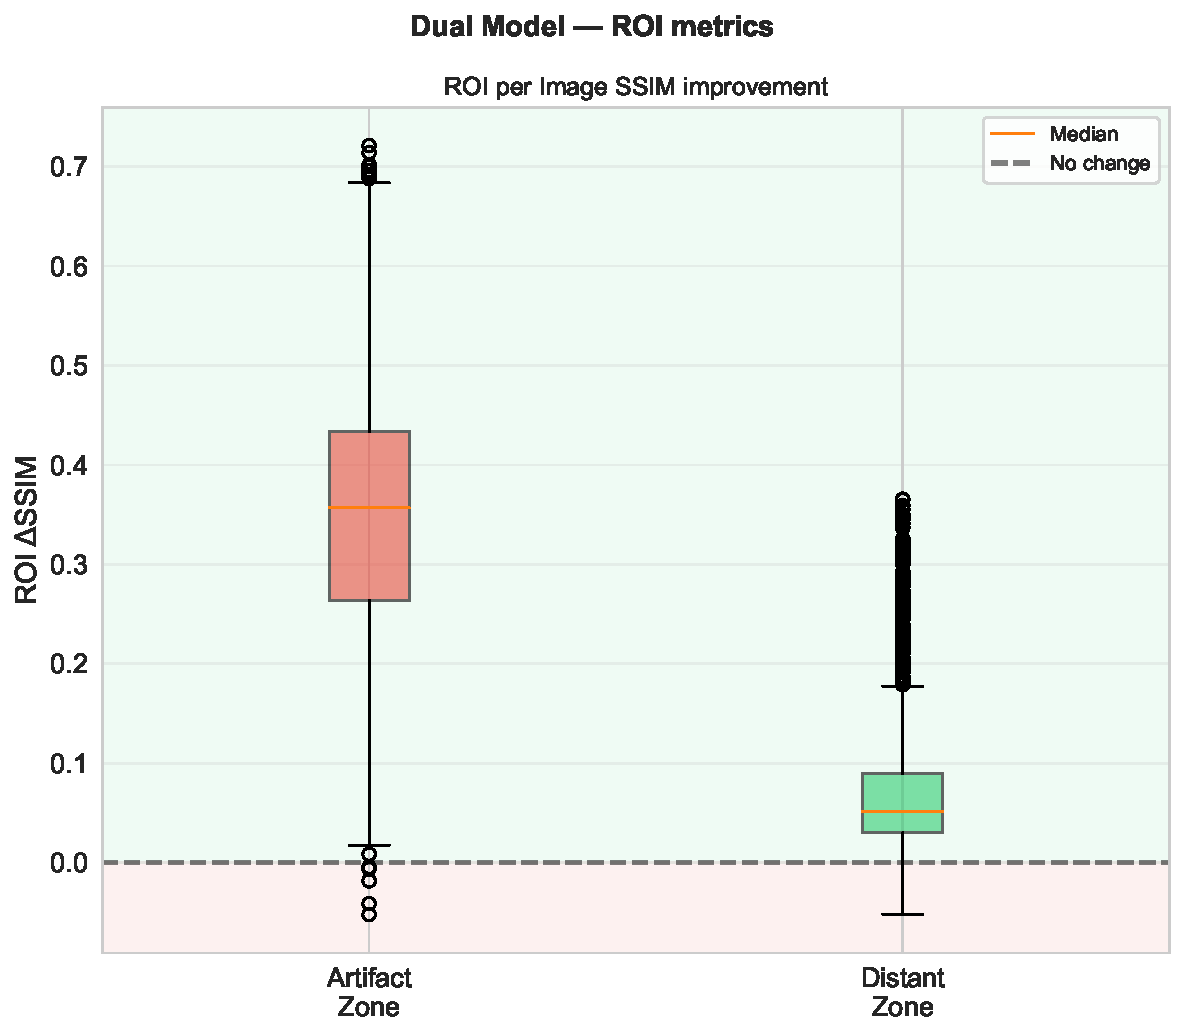
\includegraphics[width=0.95\linewidth]{Figures/Generated/evaluation/boxplot-roi-delta-ssim-fcb9fde9.pdf}
\graphiccaption[ROI per-image SSIM improvement]{Distribuicao de metricas e analise de correlacao: \texttt{boxplot\_roi\_delta\_ssim.pdf}.}
\end{figure}

\begin{figure}[htbp]
\centering
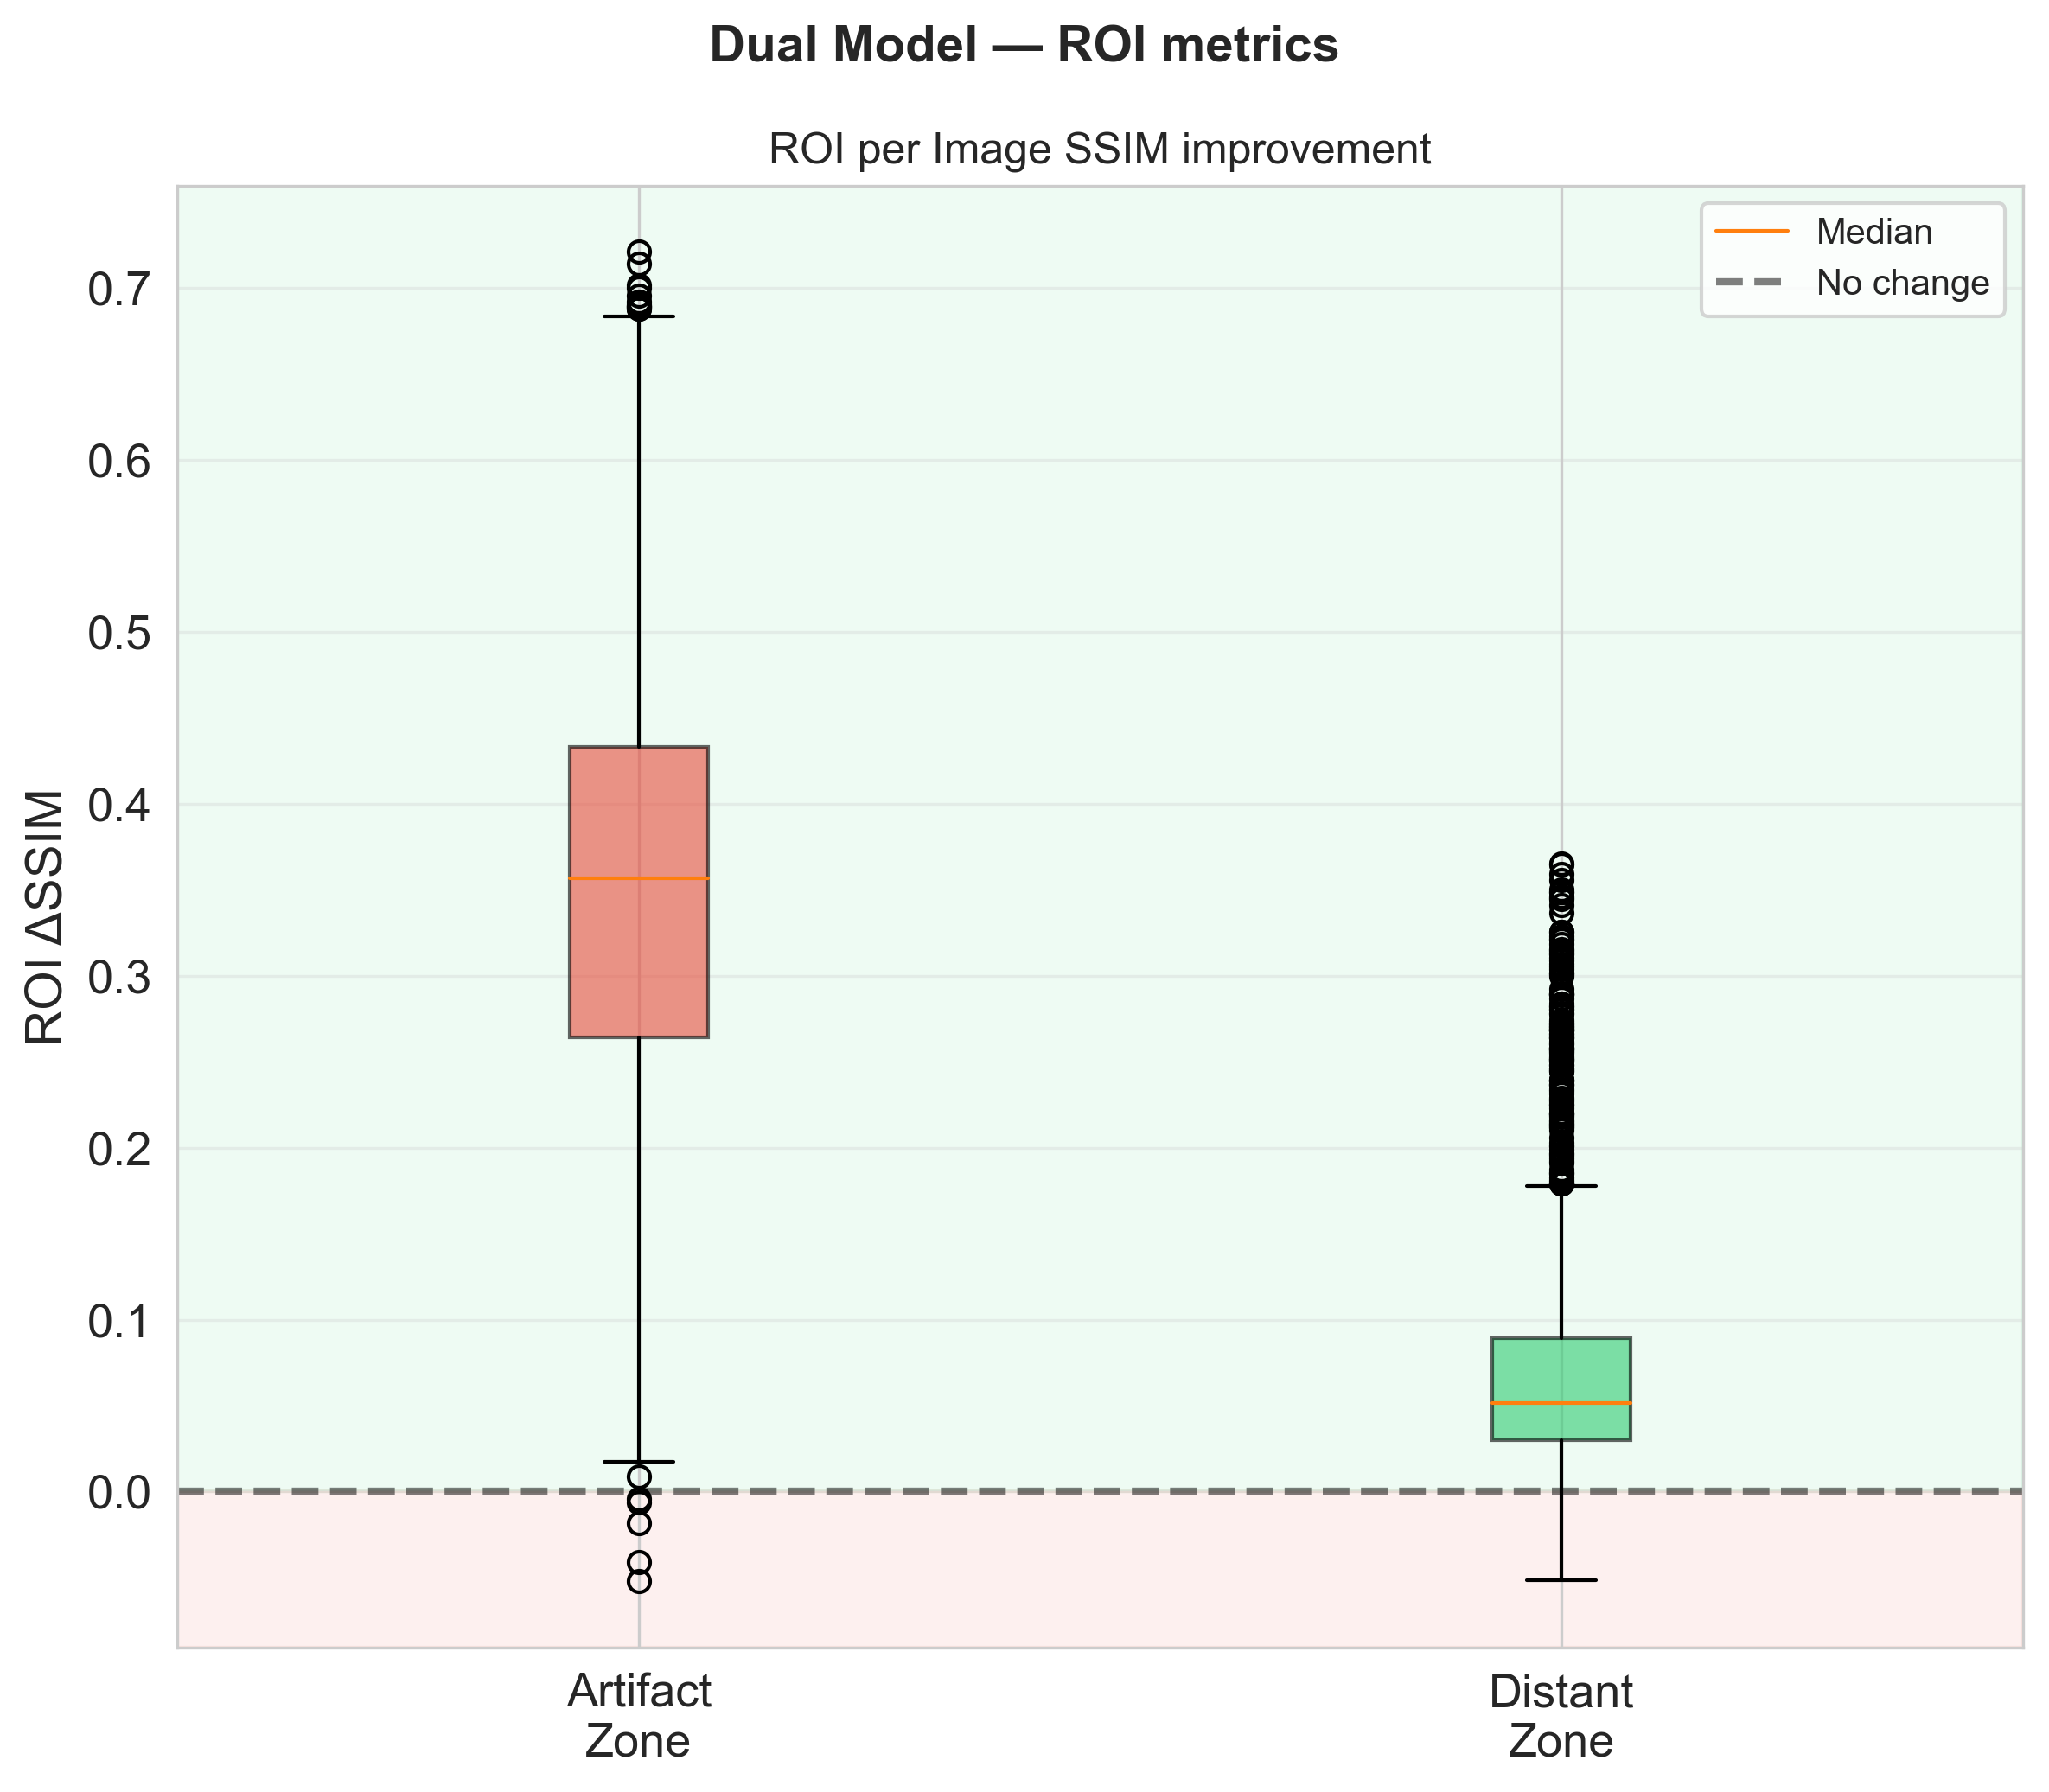
\includegraphics[width=0.95\linewidth]{Figures/Generated/evaluation/boxplot-roi-delta-ssim-577df2fe.png}
\graphiccaption[ROI per-image SSIM improvement]{Distribuicao de metricas e analise de correlacao: \texttt{boxplot\_roi\_delta\_ssim.png}.}
\end{figure}

% 20 additional copied figure(s) are intentionally not inserted automatically.
